\documentclass[12pt, a4paper]{article}
\usepackage[T1]{fontenc}
\usepackage{amsmath, listingsutf8, mathtools}
\usepackage{hyperref}
\usepackage{breakurl}
\usepackage{graphicx}
%\hypersetup{}
%\lstset{numbers=left}
\title{Exploring Compiler Optimization Techniques}
\author{A. D. Blom}
\date{}

\begin{document} \sloppy
  \maketitle
  \begin{abstract}
In this era of global digitalization, the need for performant software is larger
than ever. For the production of fast software not only 
fast hardware and solidly written code are needed, but also a well-optimizing 
compiler. This paper explores some common optimization techniques based on an 
SSA intermediate language.
  \end{abstract}

  \section{Introduction}
When a compiler translates code from a programming language to assembly languages,
it may apply a number of transformations to the source code, most often to make
programs faster (but also to enhance debugging capabilities for example). Doing
so is called code optimization.

Code optimization is most often done by first translating the source code
(as read by a \textit{lexer} and interpreted by a \textit{parser}) into an
\textit{intermediate form}, which is subsequently converted into
assembly.\cite[chapter~2]{dragon}
Such an intermediate form must be designed in such a way that it can be analyzed and
optimized easily. Such a intermediate form commonly consists of a
list of instructions (using so-called \textit{three-way address code}) grouped
into \textit{basic blocks}. Each basic block has one starting point and one
end-point. The endpoint is always a \textit{terminal instruction}
which causes control flow to leave the block (\verb+jmp+, \verb+split+, \verb+ret+
and \verb+leave+ in the intermediate form used here).

The following C source code:

\begin{lstlisting}
int sub(int a, int b)
{
	return a - b;
}
\end{lstlisting}

May be converted (by the \textit{front-end}) into the following intermediate form
(this intermediate form is described in section~\ref{sec:irused}):

\begin{lstlisting}
global int (int, int)* @sub(int p0, int p1) {
L0:	int* t1 = alloca(int);
	int* t2 = alloca(int);
	store(t1, p0);
	store(t2, p1);
	int t3 = load(t1);
	int t4 = load(t2);
	int t5 = sub(t3, t4);
	ret(t5);
L1:	leave();
}
\end{lstlisting}

Which is subsequently optimized (by the \textit{middle-end}):

\begin{lstlisting}
global int (int, int)* @sub(int p0, int p1) {
L0:	int t1 = sub(p0, p1);
	ret(t1);
}
\end{lstlisting}

And converted into assembly (by the \textit{back-end}):

\begin{lstlisting}
	.globl	sub
sub:
	movl	%edi, %eax
	subl	%esi, %eax
	ret
\end{lstlisting}

It is then that the job of the compiler is done, and the assembler takes over,
and converts the assembly into numerical codes (\textit{"ones and zeroes"}):

\begin{lstlisting}
89 66 66 f8 f0 29 00 c3
\end{lstlisting}

One may ask oneself how the intermediate code is optimized from the first into
the significantly faster second format, and how this is implemented concretlely
in software. The \textit{acc} project was written to find out, and this article
describes some of the optimization techniques used by acc (and a few more).

  \section{Intermediate representation used}
  \label{sec:irused}
The intermediate representation (IR) used here is based on the \textit{static
single assignment} (SSA) principle: every temporary variable may be assigned to
only once. It is partially based on the LLVM IR as described by~LLVM~\cite{llvm_ir}.
There are a few differences: the IR used here  uses a typesystem analogous to
C's, and uses a C-like syntax for textual 
representation as well.

The custom IR used also lacks implicit blocks, so blocks are declared 
explicitly using labels, and follow temporary value numbering.

Concretlely, the following LLVM snippet:

\begin{lstlisting}
	%1 = add i32 1, i32 2
	%2 = icmp eq i32 %1, i32 3
	br i1 %2, label %3, label %0
	ret i32 0
\end{lstlisting}

Is equivalent to the following custom-IR:

\begin{lstlisting}
L0:	int t1 = add((int)1, (int)2);
	_Bool t2 = cmp eq(t1, (int)3);
	split(t2, L3, L0);
L3:	ret((int)0);
\end{lstlisting}

Both languages feature an \verb+undef+ constant, with the ability to take on any
value. The custom IR lacks a \verb+null+ constant, it uses \verb+0+ instead.

A working C front-end is expected to be present, and snippets here will be 
either in custom IR or C.

\subsection{Common instructions}
A lot of the instructions are taken from LLVM. The non self-explanatory ones
behave as described below.
\subsubsection{alloca}
Allocates memory of the specified type, and returns a pointer to that memory.
The memory is deallocated when the function returns.
\subsubsection{split}
A conditional jump, \verb+split(a, b, c);+ jumps to \verb+b+ if \verb+a+, and
\verb+c+ if not.
\subsubsection{leave}
In a function returning \verb+T+, \verb+leave();+ is equivalent to
\verb+ret((T)undef);+. It returns from a function but returns no useful value.

  \section{SSA conversion optimization}
  \label{sec:ssa}
  \subsection{Problem}
Imperative languages usually allow variables and memory to be rewritten. SSA 
inherently, does not allow temporary variables to change their value over time. 
SSA supports several ways to support this model. One is using the \verb+alloca+
instruction to allocate memory and use the \verb+load+/\verb+store+ system,
another, is cleverly using SSA and its $\phi$ nodes. The first translation uses
rewritable memory and is therefore not a strict SSA representation of control
flow.\footnote{The intermediate form used is still SSA compliant, however, even though it
allows rewriting of \textit{memory}. The temporary values (t1 etc.) are
still single-assignment. Allowing rewritable memory is a necessary evil for
imperative languages.}

Consider the following imperative code:

\begin{lstlisting}
	int i;
	if (condition)
		i = 0;
	else
		i = 1;
	return i;
\end{lstlisting}

A naive translation would be:

\begin{lstlisting}
L0:	int* t1 = alloca(int);
	split(cond, L2, L3);
L2:	store(t1, (int)0);
	jmp(L4);
L3:	store(t1, (int)1);
	jmp(L4);
L4:	int t5 = load(t1);
	ret(t5);
\end{lstlisting}

It involves two memory accesses and a memory allocation. Pointers are involved
so it's hard to optimize any further.

It also complicates register allocation a great deal. The allocator now not 
only needs to keep track of where its temporaries are, but also the registers 
used by the \verb+alloca+ instructions. Furthermore it's complicated by 
requiring a new lifetime analysis method, instead of the one already provided 
for temporaries, since most \verb+alloca+ memory needn't be alive for the 
entirety of the surrounding function.

For further optimization it's far more convenient to turn such a complex system
with \verb+alloca+, \verb+load+ and \verb+store+ into an pure system where each
variable is truly written to once.

SSA features a mechanism that allows selecting a value based on the previously 
run block. This system is a $\phi$ node system, where a $\phi$ node is an
instruction taking a map of blocks and expressions, selecting the appropriate
expression based on the predecessing block.

\begin{lstlisting}
L0:	split(cond, L1, L2);
L1:	jmp(L3);
L2:	jmp(L3);
L3:	int t4 = phi(	L1, (int)0,
			L2, (int)1	);
	ret(t4);
\end{lstlisting}

Sometimes for imperative languages it is impossible to use the second system, 
for example in the case where actual memory is required:

\begin{lstlisting}
	int i = 0;
	foo(&i);
	return i;
\end{lstlisting}

Can't use a $\phi$ node system, since it needs \verb+i+ to actually exist in 
memory. It is therefore hard for a front-end to decide which system to use, and 
many\footnote{At least clang does so: \textit{echo "void foo() \{ int a; \}" |
 clang -x c - -S -emit-llvm -o /dev/stdout}}
default to using the first system all of the time, relying on the 
middle-end to optimize it into an SSA system. If an \verb+alloca+ 
variable can convert its \verb+load+/\verb+store+ system it shall be considered 
\textit{SSA-capable}.

\subsection[Implementation] {Implementation\footnote{This is the o\_phiable() optimization pass in opt.c in acc} }
Given a simple, one-block SSA graph:

\begin{lstlisting}
L0:	int* t1 = alloca(int);
	store(t1, (int)0);
	int t2 = load(t1);
	int t3 = add(t1, (int)10);
	store(t1, t3);
	int t4 = load(t1);
	ret(t4);
\end{lstlisting}

Can \verb+t1+ be considered SSA-capable? It's been established that an \verb+alloca+ system 
is not SSA-capable if the memory is actually required to exist. This means (naively) 
that a system is not SSA-capable if the \verb+alloca+ instruction is used outside 
its own \verb+load+/\verb+store+ instructions: that is if it is ever used in an 
instruction, except as the first operand of a \verb+store+ or \verb+load+.

\verb+t1+ meets the phiability requirements. \verb+load+ instructions need to be 
replaced by its last \verb+store+. This means that the \verb+load+ in line 3 
(\verb+t2+) needs to be replaced by its last stored value (line 2). \verb+t4+ 
similarly needs to be replaced by \verb+t3+:

\begin{lstlisting}
L0:	int t1 = add((int)0, (int)10);
	ret(t1);
\end{lstlisting}

This constitutes an enormous code shrinkage, and will speed up the code 
immensely.

Finding the last store is trivial for these one-block examples, it is more 
involved when considering a piece of code where the last store is in one of a 
\verb+load+'s block predecessors. Consider this:

\begin{lstlisting}
L0:	int* t1 = alloca(int);
	split(cond, L2, L3);
L2:	store(t1, (int)0);
	jmp(L4);
L3:	store(t1, (int)1);
	jmp(L4);
L4:	int t5 = load(t1);
	ret(t5);
\end{lstlisting}

For the load in line 7 for example, finding the last store is non-trivial, it 
has in fact got multiple last \verb+store+ instructions, one in \verb+L2+ and one in 
\verb+L3+. It is now actually required to implement a  $\phi$ node. It selects 
the value from \verb+L2+ if that was its predecessor, and the store from \verb+L3+ if 
that was its predecessor using a $\phi$ node:

\begin{lstlisting}
L0:	split(cond, L1, L2);
L1:	jmp(L3);
L2:	jmp(L3);
L3:	int t4 = phi(L1, (int)0, L2, (int)1);
	ret(t4);
\end{lstlisting}

It is also possible for an \verb+alloca+ to be loaded without any previous 
\verb+store+. In that case, the value of the \verb+load+ is undefined, and it is 
tempting to use the \verb+undef+ constant. It is important, however, that the 
result of the load is guaranteed to remain constant. That isn't the case if all 
instances are replaced by individual \verb+undef+ constants. Consider, for 
instance, the following example:

\begin{lstlisting}
L0:	int* t1 = alloca(int);
	int t2 = load(t1);
	int t3 = load(t1);
	_Bool t4 = cmp eq(t2, t3);
	...
\end{lstlisting}

The value of \verb+t4+ is well-defined, because the value of \verb+t1+ is
guaranteed not to alter spontaneously. If the following translation would be 
used:

\begin{lstlisting}
L0:	_Bool t1 = cmp eq((int)undef, (int)undef);
	...
\end{lstlisting}

The result of the comparison is undefined as well.

It is therefore required to introduce a \verb+undef+ instruction. The code would 
therefore be
optimized into:

\begin{lstlisting}
L0:	int t1 = undef(int);
	_Bool t4 = cmp eq(t1, t1);
	...
\end{lstlisting}


\section{Constant folding}
\label{sec:cfld}
\subsection{Problem}
When a programmer writes something along these lines:

\begin{lstlisting}
	int i = 10 - 3 * 2;
\end{lstlisting}

The compiler can be expected to see that i should be initialised to four, rather 
than having it emit instructions for each mathematical operation. Moreover, if a 
programmer types:

\begin{lstlisting}
	int a = 10;
	int b = a * 2;
\end{lstlisting}

The compiler can also be expected to simplify the initialisation of b into an 
initialisation to twenty. Although perhaps trivially optimised manually, these
types of trivial constant expressions occur not so much in manually written code,
but quite often in macro expansions.

Therefore the compiler may not expect all constants to be simplified as much as
possible. Instead, the compiler evaluates these constants in a process known as 
constant folding, and subsequently propegates these constants further, filling 
them in for SSA variables along the way in a process known as constant 
propagation.

\subsection[Implementation] {Implementation\footnote{This is the o\_cfld() optimization pass in opt.c in acc} }
In order to perform any useful consant folding, the compiler needs to fill in 
constants for variables where possible, so code of the form:

\begin{lstlisting}
	int a = 10;
	int b = a * a;
	return b - a;
\end{lstlisting}

Becomes:

\begin{lstlisting}
	int b = 10 * 10;
	return b - 10;
\end{lstlisting}

Once the value of \verb+b+ is determined, it should then also be filled in, to fold 
further. Since the value of \verb+b+ is 100, it can be used to fill in the return 
expression:

\begin{lstlisting}
	return 100 - 10;
\end{lstlisting}

This value can then be folded once more to yield the value 90:

\begin{lstlisting}
	return 90;
\end{lstlisting}

This algorithm might look quite involved, but its simplicity is actually 
staggering. It simply depends on SSA conversion optimization (as described in
section~\ref{sec:ssa}). SSA conversion 
optimization fills in constants for variables automatically. Consider the first 
fragment's IR before SSA conversion optimization:

\begin{lstlisting}
L0:	int* t1 = alloca(int);
	int* t2 = alloca(int);
	store((int)10, t1);
	int t3 = load(t1);
	int t4 = load(t1);
	int t5 = mul(t3, t4);
	store(t5, t2);
	int t6 = load(t2);
	int t7 = load(t1);
	int t8 = sub(t6, t7);
	ret(t8);
\end{lstlisting}

The variables still exist in their crude memory form. However, their values are 
propagated automatically once SSA conversion optimization occurs:

\begin{lstlisting}
L0:	int t1 = mul((int)10, (int)10);
	int t2 = sub(t1, (int)10);
	ret(t2);
\end{lstlisting}

The constants can now be propagated with a pass that scans for computable 
instructions (arithmetic instructions of which both operands are constants) and 
computes their values, filling them in for all future occurrences:

\begin{lstlisting}
L0:	ret((int)90);
\end{lstlisting}

\subsection{Considerations}
\subsubsection{Platform incompatibilities}
There is a way compiler-based constant folding might stand in the way of the 
programmer. Mostly the compiler can do this when folding
away instructions  operating on floating point operands, because different targets may compute 
floating point operations differently. Therefore cross-compilation becomes an 
issue; if a floating point instruction for target $Y$ normally yielding $V_y$, it 
yields $V_x$ when folded away by target $X$, causing different semantics before and 
after optimization.\cite{cfld_cross}

A solution to this problem is to implement a floating point virtual machine for 
several targets, that use non IEEE floating point. Targets using IEEE floating 
point can use C99's internal way of computing IEEE floating point operations.
Since implementing such a system is non-trivial, code duplication needs to be 
avoided. If any other optimization would need to be able to calculate an 
operation on two constants, it should run the same code. Therefore, the actual 
folding computations are performed outside of the optimiser, by a separate 
folding system.


\section{Constant split removal}
\label{sec:uncsplit}
\subsection{Problem}
After constant folding, some \verb+split+ instructions may branch on a constant
condition:

\begin{lstlisting}
La:	...
	split((_Bool)1, Lb, Lc);
Lb:	ret((int)0);
Lc:	ret((int)1);
\end{lstlisting}

Could be converted easily into:

\begin{lstlisting}
La:	...
	jmp(Lb);
Lb:	ret((int)0);
Lc:	ret((int)1);
\end{lstlisting}

This has only minor implications for further flow, except that it removes a
predecessor from block \verb+Lc+. The only way that that affects SSA validity is
that a block-expression pair may need to be removed from $\phi$ nodes in
\verb+Lc+.

Removing this predecessor may also have implications for further block inlining;
if a block has only one predecessor and the predecessor has only one successor,
the block could be merged with its predecessor.

\subsection[Implementation] {Implementation\footnote{This is the o\_uncsplit() pass in opt.c acc} }
The implementation of this optimization simply needs to check whether the first
parameter of a \verb+split+ instruction is constant, and convert it into a
\verb+jmp+ accordingly. It also needs to check for the presence of $\phi$ nodes
in the block not covered by the \verb+jmp+ instruction, and remove them accordingly:

\begin{lstlisting}
La:	...
	split((_Bool)1, Lb, Lc);
Lb:	...
Lc:	int tA = phi(La, (int)10, ...);
	...
\end{lstlisting}

Needs to get rid of the \verb+La+ items from the \verb+tA+ $\phi$ node too:

\begin{lstlisting}
La:	...
	jmp(Lb);
Lb:	...
Lc:	int tA = phi(...);
	...
\end{lstlisting}


\section{Block inlining}
\subsection{Problem and implementation}
When a block has only one predecessor and its single predecessor
also has one successor, its instructions can be inlined into the block it succeeds:

\begin{lstlisting}
L0:	...
	jmp(L1);
L1:	int t2 = add((int)0, (int)1);
	jmp(L3);
L3:	...
\end{lstlisting}

Becomes (assuming L1 has no other predecessors):

\begin{lstlisting}
L0:	...
	int t1 = add((int)0, (int)1);
	jmp(L2);
L2:	...
\end{lstlisting}

That way the amount of jumps and blocks is reduced without duplicating instructions.

It's a very trivial optimization but occurs quite a lot, especially considering
the front-end may generate redundant blocks all the time. Consider an infinite
\verb+for+ loop:

\begin{lstlisting}
	for (; cond;)
		;
\end{lstlisting}

The front-end puts the initialization clause in the block it's currently writing
to, but generates a new block for the condition, then generates (without knowledge
of the loop body) a block for the final loop clause (this block is needed to jump
to when compiling a \verb+continue+ statement). It inserts this block after
it has generated the body block.

This would therefore be a possible translation:

\begin{lstlisting}
	/* enter the loop */
L0:	jmp(L1);
	/* continue or break from the loop */
L1:	split(cond, L2, L4);
	/* go to the final clause */
L2:	jmp(L3);
	/* no final clause, jump to loop start */
L3:	jmp(L1);
L4:	...
\end{lstlisting}

It can be noticed quite easily that \verb+L3+ only has one predecessor (\verb+L2+), and its
predecessor only one successor. It can therefore be merged with \verb+L2+:

\begin{lstlisting}
	/* enter the loop */
L0:	jmp(L1);
	/* continue or break from the loop */
L1:	split(cond, L2, L3);
	/* go to the final clause */
	/* no final clause, jump to loop start */
L2:	jmp(L1);
L3:	...
\end{lstlisting}

This turns out to be quite an interesting case, however; it can also be noticed
that this example might be optimized further, so the \verb+split+ in \verb+L1+
jumps to itself immediately. This is because \verb+L2+ is empty besides the \verb+jmp+
instruction: the condition for empty loops to be inlined is therefore more relaxed.

In fact, all empty blocks (except \verb+L0+ and empty blocks that are their own predecessor) can be inlined:

\begin{lstlisting}
L0:	jmp(L1);
L1:	split(cond, L1, L2);
L2:	...
\end{lstlisting}

\section{Block pruning}
\label{sec:prune}
\subsection{Problem}
When the intermediate form is generated by the front-end, it may leave blocks in
the IR without any predecessors. This is often the result of a language that
allows the programmer to write unreachable code. I.e. the following C:

\begin{lstlisting}
return 0;
return 1;
\end{lstlisting}

There's no was the second line could possibly be reached, and this is even obvious
in the intermediate form. This would be a possible naive translation:

\begin{lstlisting}
L0:	ret((int)0);
L1:	ret((int)1);
\end{lstlisting}

The \verb+L1+ block can be left out in its entirety, improving code size.

\subsection[Implementation]{Implementation\footnote{A reference implementation
can be found in acc as the o\_prune() pass} }
A block can be left out if it has no predecessors and isn't \verb+L0+.
This is a fairly trivial operation. The only consideration might be a $\phi$
node in one of the block's successors. If such a successor has a $\phi$ node with
an item for the block marked for removal, that item must be removed. That's
always the case, however, when removing a block.

  \section{Register allocation}
  \label{sec:regalloc}
  \subsection{As an optimization}
It's hard to categorize register allocation as either an optimization or a
general method used in assembly generation. For the purposes of this article
it'll be classified as the former, because it is a way to speed up generated
assembly.

\subsection{Problem}
CPUs have only a limited amount of registers. The original i386 processors had
only six general purpose registers for example (\verb+eax+, \verb+ebx+, \verb+ecx+,
\verb+edx+, \verb+esi+ and \verb+edi+).\cite[section~3.4.1]{intel} It is
therefore required that these registers are used cleverly to house variables\footnote{The
results of SSA instructions aren't variables strictly speaking, but for the sake
of this section they will be regarded as variables.}, so
as little as possible performance is lost due to the inherent slowness of stack
memory.

\subsection{Implementation}
\subsubsection{Restricter}
First the IR is handed over to a target-specific \textit{restricter}. This
restricter makes sure the IR meets certain platform requirements (i.e.
putting an integral/pointer return value in \verb+eax+ on x86 systems).
Making sure register requirements are met are done with the \verb+mov+ instruction.
The \verb+mov+ instruction copies another instruction result, but has a separate
life, and therefore lifetime. The \verb+mov+ result is \textit{tagged}
(annotated in the IR) with a location (\verb+loc+) tag, specifying the register.

\subsubsection{Register allocator}
To make a selection of variables to which registers can be assigned, variable
usage frequency is the most important factor. It is therefore important to
have an analysis pass analyzing variable usage frequency. A simple technique
is to simply count the amount of instructions in which the variable is used. This
disregards any control flow (and therefore block execution repetition). Such
an analysis is trivial.\footnote{This is the a\_used() analysis in analyze.c.}

A variable's lifetime needs to be considered as well. After all, no two
variables that are alive simultaneously may be assigned the same register. The
lifetime analysis step is a bit more involved, but relies on the basic principle
that a variable's lifetime starts at definition, and ends at its last usage. Its
last usage is the usage after which control can't ever reach a usage
again.\footnote{This is the a\_lifetime() analysis in analyze.c.}

Consider variable lifetimes for this block:

\begin{lstlisting}
L0:	int t1 = mul((int)2, (int)3);
	int t2 = add(t1, (int)1);
	int t3 = div(t1, t2);
	int t4 = mul(t1, t2);
	int t5 = sub(t3, t4);
	ret(t5);
\end{lstlisting}

By the target (x86) restricter, the following restrictions are made:

\begin{lstlisting}
L0:	int t1 = mul((int)2, (int)3);
	int t2 = add(t1, (int)1);
	int t3 = div(t1, t2);
	int t4 = mul(t1, t2);
	int t5 = sub(t3, t4);
	/* loc(r0) */
	int t6 = mov(t5);
	ret(t6);
\end{lstlisting}

During lifetime analysis, the following observations are added:

\begin{lstlisting}
L0:	int t1 = mul((int)2, (int)3);
	int t2 = add(t1, (int)1);
	int t3 = div(t1, t2);
	/* endlife(t1, t2) */
	int t4 = mul(t1, t2);
	/* endlife(t3, t4) */
	int t5 = sub(t3, t4);
	/* loc(r0), endlife(t5) */
	int t6 = mov(t5);
	/* endlife(t6) */
	ret(t6);
\end{lstlisting}

Such lifetime observations may be graphed into the overlap graph as shown in
figure~\ref{fig:ovl}.

\begin{figure}[h]
\begin{center}
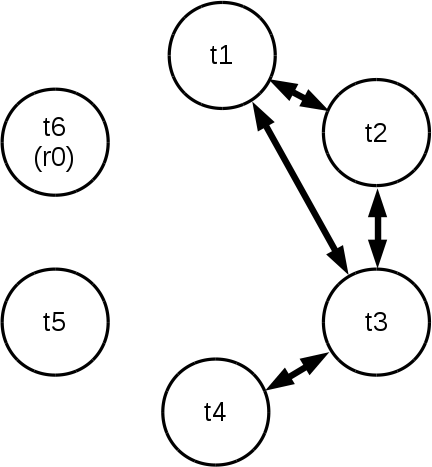
\includegraphics[resolution=128]{ovldump.png}
\caption{Variable overlap graph. An arrow indicates a lifetime overlap.}
\label{fig:ovl}
\end{center}
\end{figure}

From this, certain registers can be induced further. There is no overlap
between \verb+t6+ and the variable it \verb+mov+s (\verb+t5+). Therefore
\verb+t5+ is also hinted to be placed into \verb+r0+.

All variables hinted towards being placed in a certain location are put there
when possible. Sometimes hints may overlap, in which case the most frequently
used is picked. The situation becomes as shown in figure~\ref{fig:ovl_ind}.

\begin{figure}[h]
\begin{center}
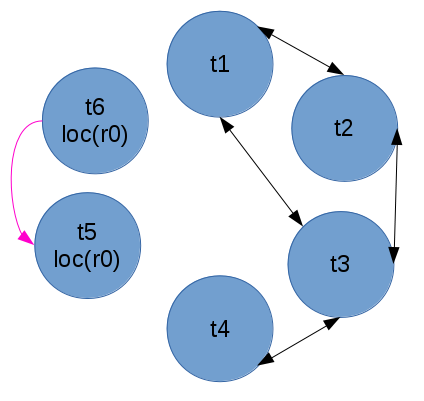
\includegraphics[resolution=128]{ovldump_ind.png}
\caption{Variable overlap graph after induction.}
\label{fig:ovl_ind}
\end{center}
\end{figure}

The remaining registers are allocated per variable in lexical order. If there
aren't enough registers available, the least frequently used are stored in memory.
Here, \verb+t1+ and \verb+t4+ are put in \verb+r0+, \verb+t2+ is put in \verb+r3+
and \verb+t3+ is put in \verb+r1+. These registers are \verb+eax+, \verb+edx+ and
\verb+ebx+ respectively. \verb+r3+ is chosen instead of \verb+r1+, because
\verb+r1+ is callee-save in the used calling convention (GNU i386). Caller-saved
registers are preferred over callee-saved registers because they have less
function prologue/epilogue overhead: they needn't be stored when entering the
function and restored when leaving the function.

The following tags are the result of register allocation based on these principles:

\begin{lstlisting}
L0:	/* loc(r0) */
	int t1 = mul((int)2, (int)3);
	/* loc(r3) */
	int t2 = add(t1, (int)1);
	/* loc(r1) */
	int t3 = div(t1, t2);
	/* endlife(t1, t2), loc(r0) */
	int t4 = mul(t1, t2);
	/* endlife(t3, t4), loc(r0) */
	int t5 = sub(t3, t4);
	/* loc(r0), endlife(t5) */
	int t6 = mov(t5);
	/* endlife(t6) */
	ret(t6);
\end{lstlisting}

The step of generating assembly is now only trivial.

\section{Conclusion}
There are many ways IR can be optimized into a faster form. These have been
examples of ways to do so, there are, however, many more. Most of these
optimizations have seen a practical implementation in the included \textit{acc}
software, for reference and practical examples. In appendix~\ref{sec:accdet} parts
of this software are described in detail.

\begin{thebibliography}{9}
  \bibitem{dragon} Aho et al.
  \emph{Compilers: Principles, Techniques And Tools}.
  (1988)

  \bibitem{llvm_ir}
  \emph{LLVM Language Reference Manual}. (2014) Consulted on 2014/11/11,
  \url{http://llvm.org/docs/LangRef.html}

  \bibitem{cfld_cross}
  \emph{Constant folding and cross compilation}. (s.d.) Consulted on 2014/11/11,
  \url{http://en.wikipedia.org/wiki/Constant_folding#Constant_folding_and_cross_compilation}

  \bibitem{intel}
  Intel Corporation.
  \emph{Intel\textregistered{} 64 and IA-32 Architectures Software Developer's
Manual Volume~1}.
  (2014)

\end{thebibliography}


\newpage
\appendix
\section{Implementation Details for acc}
\label{sec:accdet}
\subsection{Introduction}
  \textit{acc} (the antonijn/Antonie C Compiler) is a software project with the intent of
one-day being self-hosting (able to compile itself). The only external library
it depends on is the C99 standard library, and it's written in portable standard C99.

  acc implements many of the optimizations mentioned in the main paper, and could
serve as a reference implementation for them. It is however, much more than that,
of course, since it has to provide not only an optimizer, but back-ends and a C
front-end as well. Only the subsystems relevant to compiler optimization are
described here in detail. The most relevant subsystem is the so-called
\textit{intermediate} subsystem (shortened to \verb+itm+ in code), implementing
functions and data structures for defining and manipulating an intermediate form
SSA tree. It also implements functions for writing such a tree to a file in text
form.

  \subsection{Object oriented programming}
Although the C language doesn't natively feature object oriented syntax, it doesn't
exclude the possibility of writing clean object oriented code.

\begin{figure}[h]
\begin{center}
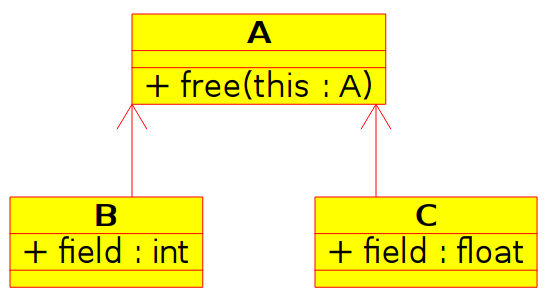
\includegraphics[resolution=256]{ABC.png}
\caption{Class diagram example}
\label{fig:abc}
\end{center}
\end{figure}

The class diagram described in figure~\ref{fig:abc} could be implemented in
C as follows:

\begin{lstlisting}
struct A {
	/* pointer to a B or C object */
	void *extended;

	void (*free)(struct A *self);
};

struct B {
	struct A base;

	int field;
};

struct C {
	struct B base;

	float field;
};
\end{lstlisting}

This style will be found a lot in the acc source code, although sometimes
missing the \verb+extended+ field in a base class (in which case the addresses
of both types are presumed compatible).

  \subsection{The AST and its elements}
The \verb+itm+ abstract syntax tree (AST) is not very complex. It mostly uses
linked lists (the \verb+struct list *+, for instance, is a linked list containing
only \verb+void *+ instances) for chaining instructions and blocks together.

A variety of structures is needed to store the following snippet internally:

\begin{lstlisting}
global int (int, int)* @gcd(int p0, int p1) {
L0:	jmp(L1);
L1:	int t2 = phi(L0, p0, L5, t7);
	int t3 = phi(L0, p1, L8, t9);
	_Bool t4 = cmp neq(t2, t3);
	split(t4, L6, L10);
L5:	_Bool t6 = cmp gt(t2, t3);
	int t7 = sub(t2, t3);
	split(t6, L1, L8);
L8:	int t9 = sub(t3, t2);
	jmp(L1);
L10:	ret(t2);
}
\end{lstlisting}

And AST capable of storing such an IR, must be able to store functions, global
variables (unimplemented as of yet), basic blocks, instructions, parameters
(unimplemented as of yet), literals and \verb+undef+ constants. These elements
are implemented through a structure system as described in figure~\ref{fig:ast}.

\begin{figure}[h]
\begin{center}
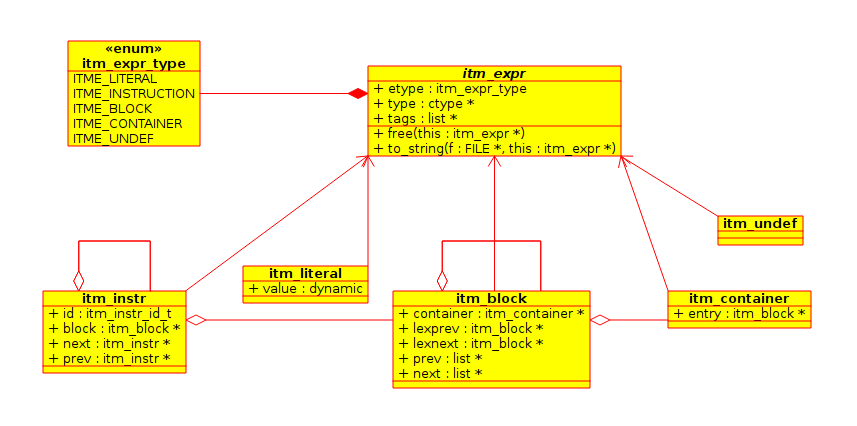
\includegraphics[resolution=150]{ast.png}
\caption{The AST class diagram}
\label{fig:ast}
\end{center}
\end{figure}

A common base type for most AST elements is \verb+struct itm_expr+ (the
expression base type). It contains a destructor, a (C) typename, and a list of
\textit{tags}. Tags are used to store expression attributes (\textit{"tag"}).
Tags are used in section~\ref{sec:regalloc} for example.

\begin{lstlisting}
struct itm_expr {
	/* derived type identifier
	 *
	 * The enumeration contains for
	 * example:
	 *  ITME_INSTRUCTION,
	 *  ITME_LITERAL
	 *  ITME_BLOCK
	 *  ...
	 */
	enum itm_expr_type etype;

	/* expression's C typename */
	struct ctype *type;
	/* tag list */
	struct list *tags;

	/* destructor
	 * (implemented by derived class) */
	void (*free)(struct itm_expr *e);
	/* to_string for file dumps
	 * (implemented by derived class) */
	void (*to_string)(FILE *f, struct itm_expr *e);
};
\end{lstlisting}

Global variables (as of yet unimplemented) and functions are represented through
\textit{container} structures (\verb+struct itm_container *+). They contain an
entry block, and are expressions themselves (as required to be called):

\begin{lstlisting}
struct itm_container {
	/* expression base */
	struct itm_expr base;

	/* container identifier */
	char *id;
	/* entry block */
	struct itm_block *block;
};
\end{lstlisting}

Blocks are represented through \verb+struct itm_block *+ structures. They are
expressions (as required to be a parameter to \verb+jmp()+ or \verb+split()+),
contain a pointer to the first instruction, the last instruction (terminal
instruction), a pointer to the block that's lexically next (\verb+L1+ for
\verb+L0+ in the first example), a pointer to the block that's lexically previous
(\verb+L0+ for \verb+L1+ in the first example, \verb+NULL+ for \verb+L0+),
and two lists of blocks that are sementically next and previous (\verb+L1+ is
\verb+L10+'s semantic predecessor, for example).

\begin{lstlisting}
struct itm_block {
	/* expression base */
	struct itm_expr base;

	/* the container the block's contained by */
	struct itm_container *container;
	/* first and last instructions */
	struct itm_instr *first, *last;
	/* blocks lexically next and previous */
	struct itm_block *lexnext, *lexprev;
	/* predecessor and successor lists */
	struct list *next, *prev;
};
\end{lstlisting}

Instructions are represented as \verb+struct itm_instr+ pointers. They are
themselves a linked list: they contains pointers to the previous and next
instructions. They also link to their parent block, and have a list of their
operands. They contains a field of a strange type (\verb+itm_instr_id_t+) which
is an instruction identifier constant for each instruction type.

For instance, an instruction of the type \verb+add+ has a constructor called
\verb+itm_add()+. Its identifier can be obtained passing that function to the
\verb+ITM_ID()+ macro: \verb+ITM_ID(itm_add)+.

The structure looks roughly like this:

\begin{lstlisting}
struct itm_instr {
	/* expression base type */
	struct itm_expr base;

	/* instruction identifier (add, sub,
	 * leave, etc.) */
	itm_instr_id_t id;
	/* parent block */
	struct itm_block *block;
	/* instruction operand list */
	struct list *operands;
	/* previous and next instructions */
	struct itm_instr *prev, *next;
};
\end{lstlisting}

Then there has to be a way to store literals (both floating point and integral)
and \verb+undef+ constants. These structures are trivial:

\begin{lstlisting}
struct itm_literal {
	/* expression base */
	struct itm_expr base;

	/* value, sharing memory */
	union {
		long long i;
		double d;
		float f;
	} value;
};

struct itm_undef {
	/* expression base */
	struct itm_expr base;
};
\end{lstlisting}

\subsubsection{Type system}
The type system used by the IR is the same as the type system used by C. Few
details are of importance, but it's important that the primitive types are
represented by \verb+&cint+, \verb+&cshort+, \verb+&clong+, \verb+&cchar+,
\verb+&cbool+, \verb+&cfloat+ and \verb+&cdouble+. Type system types are of type
\verb+struct ctype *+.

\subsection{Expression constructors}
\subsubsection{Instructions}
Writing instructions to a basic block is done with an instruction constructor,
which creates an instruction and inserts it at the end of a basic block. The
instruction constructor prototype for \verb+add+ is as follows:

\begin{lstlisting}
struct itm_instr *itm_add(
	struct itm_block *parent,
	struct itm_expr *left,
	struct itm_expr *right);
\end{lstlisting}

\subsubsection{Literals}
Creating a literal is done by invoking \verb+new_itm_literal()+:

\begin{lstlisting}
struct itm_literal *new_itm_literal(
	struct itm_container *c,
	struct ctype *type);
\end{lstlisting}

After creating a new literal, its value is manipulated by setting the
\verb+value+ field. The \verb+c+ parameter is needed to register the literal
with a container, to automatically dispose
of the literal when the container is disposed of.

\subsubsection{Example}
To add an addition of literals \verb+1+ and \verb+2+ (\verb+int+s) to block
\verb+b+, one'd write:

\begin{lstlisting}
struct itm_literal *l, *r;
l = new_itm_literal(b->container, &cint);
r = new_itm_literal(b->container, &cint);
l->value.i = 1;
r->value.i = 2;

/*
 * &l->base is used instead of just l
 * because the constructor takes an
 * itm_expr *, not an itm_literal *.
 */
itm_add(b, &l->base, &r->base);
\end{lstlisting}


\subsection{Optimizations and analyzations}
Optimizations as described in sections~\ref{sec:ssa}, \ref{sec:cfld},
\ref{sec:uncsplit} and \ref{sec:prune}. Are implemented in \textit{itm/opt.c}.
They are the \verb+o_phiable()+, \verb+o_cfld()+, \verb+o_uncsplit()+ and
\verb+o_prune()+ functions respectively. SSA-capability, lifetime and usage
analyses are implemented in \textit{itm/analyze.c} as \verb+a_phiable()+,
\verb+a_lifetime()+ and \verb+a_used()+ respectively.

\subsection{Command line options}
Invoke \verb+acc --help+ to obtain information about command line options. Most
importantly, to dump the IR of the C file \verb+test.c+ into \verb+test.c.ir+, run:

\begin{lstlisting}
$ ./acc test.c -Sir
\end{lstlisting}

Add \verb+-O2+ to optimize.

Using \verb+-S+ is very unstable as of the pws-bo2 version.

\subsection{Conclusion}
This has been an insight into the inner workings of acc. The optimizations
and analyzations have been left undescribed, but have been (hopefully) written
in such a way that they can be understood easily given the information provided
before.

\end{document}
